\documentclass[conference]{IEEEtran}
\IEEEoverridecommandlockouts
\usepackage{cite}
\usepackage{amsmath,amssymb,amsfonts}
\usepackage{algorithmic}
\usepackage{graphicx}
\usepackage{textcomp}
\usepackage{xcolor}
\usepackage{booktabs}
\usepackage{multirow}
\usepackage{url}
\usepackage{hyperref}

\def\BibTeX{{\rm B\kern-.05em{\sc i\kern-.025em b}\kern-.08em
    T\kern-.1667em\lower.7ex\hbox{E}\kern-.125emX}}

\begin{document}

\title{RAG-Based Threat Memory: An Adaptive and Explainable Defense Against Indirect Prompt Injection in LLM Agents}

\author{\IEEEauthorblockN{Eman Al-Zalab}
\IEEEauthorblockA{Department of Computer Science, Sana'a University, Sana'a, Yemen\\
Email: eman.alzalab@su.edu.ye}
}

\maketitle

\begin{abstract}
Autonomous large language model (LLM) agents operating within tool-integrated environments remain inherently vulnerable to Indirect Prompt Injection (IPI), wherein adversaries embed adversarial instructions inside untrusted external content. Conventional defenses predominantly rely on static input classification or costly inference-time trajectory re-execution, requiring expensive parameter fine-tuning to assimilate emerging threats and failing to supply auditable provenance for security decisions. This paper presents RAG-Based Threat Memory (RTM), an adaptive defense middleware that externalizes dynamic threat intelligence into an updatable, non-parametric vector store. RTM couples an un-finetuned boundary detector with a dense semantic memory of verified threat exemplars through a calibrated Weighted Soft-OR fusion rule, accompanied by an evidence-extraction pipeline that attributes each containment decision to documented exemplar records. Threat adaptation is achieved via constant-time append operations without gradient updates, safeguarded by a multi-stage ingestion filter engineered to resist memory poisoning.

Evaluated across $n = 1,990$ benchmark items ($1,673$ held-out injection variants across six threat families and $317$ benign utility instances drawn from AgentDojo, InjecAgent, and BIPIA), Full RTM ($B_3$) attains an Attack Success Rate (ASR) of $6.3\%$ [95\% Wilson CI: $5.2\%$, $7.5\%$], an overall False Positive Rate (FPR) of $16.1\%$ [95\% CI: $12.4\%$, $20.5\%$], and an overall accuracy of $92.2\%$ [95\% CI: $90.9\%$, $93.3\%$]. We emphasize that while hyperparameter tuning targeted a nominal empirical $\text{FPR} \le 1.0\%$ on the calibration partition ($n=750$), the observed test partition FPR was $16.1\%$ ($51/317$ false alarms), driven predominantly by domain distribution shift on technical hard-negative interactions ($26.3\%$ on complex system and security documentation vs. $3.5\%$ on ordinary benign interactions). Rigorous paired analysis demonstrates that RTM does not surpass the standalone base detector on zero-day attacks prior to memory ingestion ($B_1$ ASR = $5.7\%$, exact McNemar $p = 0.0039$, disconfirming hypothesis $H_1$ under our frozen analysis plan). Crucially, because $B_1$ operates on raw detector score thresholding while $B_3$ applies calibrated Soft-OR fusion risk thresholding, their differing decision rules preclude isolating the empirical effect of the threat memory alone. Nevertheless, RTM provides clear operational utility: ingesting verified exemplars yields an empirical adaptation gain of $+88.9\%$ [95\% bootstrap CI: $+72.2\%$, $+100.0\%$] across an evaluated proof-of-concept subset of 18 held-out evasions with zero false alarm inflation ($\Delta\text{FPR} = +0.00\%$), indicating that certain evasive variants may be remediated without retraining (though not establishing universal remediability across arbitrary attacks); delivers $94.0\%$ explanation verification fidelity ($\kappa = 1.000$) within an audited 50-decision convenience sample with zero context leakage; and executes with a median local middleware latency of only $22.0$\,ms---operating over $78\times$ faster than standalone remote detector inference ($1719.9$\,ms) and over $50\times$ faster than trajectory re-execution defenses ($1102.9$\,ms). Code, memory exemplars, and execution traces are publicly available at \url{https://github.com/eman232001/RAG_Based-Threat-Memory}.
\end{abstract}

\begin{IEEEkeywords}
LLM agents, indirect prompt injection, retrieval-augmented defense, threat memory, adaptive security, memory poisoning, verifiable explanations, AgentDojo.
\end{IEEEkeywords}

\section{Introduction}
Autonomous software agents driven by large language models (LLMs) increasingly execute complex workflows by reading external documents, retrieving web data, and invoking application programming interface (API) tools \cite{yao2023react, schick2023toolformer}. In these architectures, retrieved data and system instructions share a unified semantic context. Consequently, untrusted external inputs can manipulate agent execution, a vulnerability formally designated as Indirect Prompt Injection (IPI) \cite{greshake2023not, owasp2025llm01}. When an agent processes untrusted content containing disguised imperatives, the model may execute attacker-specified commands, leading to unauthorized privilege escalation, sensitive data exfiltration, or destructive tool execution \cite{vassilev2025adversarial}. Empirical benchmarks such as InjecAgent \cite{zhan2024injecagent}, BIPIA \cite{yi2023benchmarking}, and AgentDojo \cite{debenedetti2024agentdojo} corroborate this vulnerability, demonstrating attack success rates exceeding 70\% against state-of-the-art models \cite{wang2025agentvigil, zhan2025adaptive}.

Contemporary defense paradigms exhibit distinct operational limitations. Architectural containment and privilege-isolation frameworks (e.g., CaMeL \cite{debenedetti2025defeating}, Progent \cite{shi2025progent}) restrict tool capabilities but do not inspect intermediate text payloads. Fine-tuned safety classifiers (e.g., Llama Guard \cite{inan2023llama}, DataSentinel \cite{liu2025datasentinel}) and instruction-hierarchy tuning \cite{wallace2024instruction} require extensive retraining to assimilate newly discovered attack vectors and generalize poorly to unseen lexical structures. Conversely, behavioral re-execution defenses such as MELON \cite{zhu2025melon} incur prohibitive computational overhead by executing dual masked trajectories, doubling token costs and generating seconds of latency per tool response. Crucially, existing detectors output scalar risk scores without evidence attribution, preventing security analysts from verifying whether an intervention stems from legitimate threat signatures or spurious semantic correlations.

To resolve these trade-offs, this paper investigates non-parametric threat externalization: rather than altering model weights, adaptive security knowledge is maintained in an external, retrieval-augmented threat memory. We introduce \textbf{RAG-Based Threat Memory (RTM)}, an adaptive defense middleware deployed at the agent's tool-return boundary. RTM unifies an un-finetuned LLM boundary detector with a dense semantic index of documented, verified injection patterns via a calibrated Weighted Soft-OR probabilistic fusion rule. When a content payload is intercepted, RTM performs sentence-level dense retrieval to compute memory similarity, scores the payload with the base detector, and derives a calibrated composite risk score. If a violation is flagged, an explanation module generates an auditable citation detailing the nearest documented threat exemplar and the exact offending text segment. Because an external memory introduces an ingestion attack surface, RTM incorporates an automated multi-stage verification pipeline to prevent adversarial memory poisoning.

The primary contributions of this work are:
\begin{enumerate}
    \item \textbf{Decoupled Defense Middleware:} We formalize the RTM architecture, which combines zero-training boundary detection with dense threat exemplar retrieval through a monotonic Weighted Soft-OR fusion formulation calibrated via isotonic regression.
    \item \textbf{Non-Parametric Threat Adaptation:} We develop a verified ingestion pipeline that incorporates newly documented attack families via constant-time vector append operations, eliminating model fine-tuning while enforcing schema-conformance and semantic non-redundancy to resist poisoning.
    \item \textbf{Verifiable Decision Provenance:} We introduce an evidence-extraction mechanism that accompanies each mitigation decision with the exact triggering sentence span and matching threat record citation, validated through independent human audits with zero protected context leakage.
    \item \textbf{Rigorous Empirical Evaluation:} Across $n = 1,990$ items ($1,673$ held-out attack variants and $317$ benign instances), Full RTM ($B_3$) attains an ASR of $6.3\%$ [95\% Wilson CI: $5.2\%$, $7.5\%$] and an FPR of $16.1\%$ [95\% CI: $12.4\%$, $20.5\%$], operating at $22.0$\,ms median local middleware latency. We report empirical hypothesis outcomes candidly under our frozen analysis plan: while zero-day containment does not exceed the standalone base detector ($B_1$ ASR = $5.7\%$, disconfirming $H_1$; a difference shaped by distinct decision rules and calibration rather than isolating memory alone), RTM provides validated adaptation on selected evasions ($+88.9\%$ gain across 18 cases, showing certain evasions are remediable), sample-conditioned explanation fidelity ($94.0\%$ EVR on 50 audited decisions), and complete ingestion poisoning resistance ($0.0\%$ MPS across 200 trials).
\end{enumerate}

\section{Problem Formulation and Threat Model}
\subsection{Problem Formulation}
Let an autonomous agent execute a task guided by user instruction $U$. During execution, tool invocations return external unstructured content $C$ (e.g., retrieved web text, emails, or database records). The content $C$ comprises an ordered sequence of sentence segments $\mathcal{S}(C) = (s_1, s_2, \dots, s_m)$. The adversary embeds an indirect prompt injection within an untrusted segment $s_j \in \mathcal{S}(C)$ to hijack agent control flow upon ingestion.

Let $\mathcal{M} = \{r_1, r_2, \dots, r_N\}$ denote the threat memory, where each record $r_i = (p_i, d_i, y_i)$ comprises an injection exemplar payload $p_i$, a structural threat description $d_i$, and an attack family label $y_i$. The objective is to construct a decision function:
\begin{equation}
D(U, C; \mathcal{M}) \rightarrow \{\text{allow}, \text{block}\}
\end{equation}
evaluated at each tool-return boundary such that: (1) adversarial content is intercepted before context integration; (2) benign task completion is preserved; (3) newly documented threats are absorbed without weight fine-tuning; and (4) every block decision is attributed to documented evidence.

\subsection{Threat Model}
We adopt the standard indirect injection threat model \cite{debenedetti2024agentdojo, zhan2024injecagent}. The adversary cannot directly modify the user instruction $U$, agent system prompts, or core model weights. However, the adversary exercises write access over external data sources retrieved by the agent's tools. The attacker's objective is to alter execution state, induce unauthorized tool calls, or exfiltrate private context.

We evaluate two distinct threat environments:
\begin{enumerate}
    \item \textbf{Static Zero-Day Injection:} The attacker deploys novel lexical variants across held-out attack families whose specific signatures are entirely absent from the initial threat memory $\mathcal{M}$.
    \item \textbf{Adaptive Black-Box Fuzzing:} The attacker inspects binary defense outcomes across repeated queries, leveraging mutation heuristics (synonym replacement, framing shifts, and structural obfuscation) to bypass detection.
    \item \textbf{Memory Poisoning:} The adversary attempts to submit malicious candidate records into the memory ingestion queue to induce false dismissals or trigger broad false alarms.
\end{enumerate}

\subsection{Formal Hypotheses}
We evaluate six pre-specified research questions and formal hypotheses governed by a post hoc frozen analysis plan (recorded in the analysis specification file \texttt{prereg.yaml} prior to final test evaluation):
\begin{itemize}
    \item \textbf{H1 (Zero-Day Containment):} On held-out attack variants, Full RTM ($B_3$) attains an ASR non-inferior or superior to the base detector alone ($B_1$) under paired McNemar testing ($\alpha = 0.05$, Holm-Bonferroni corrected).
    \item \textbf{H2 (Threat Adaptation Gain):} Upon appending a verified exemplar for a held-out threat family, ASR on that family decreases significantly ($AG > 0$, lower bound of 95\% bootstrap CI $> 0$) while benign false alarms increase by at most 1.0 percentage point ($\Delta\text{FPR} \le 1.0\text{ pp}$).
    \item \textbf{H3 (Adaptive Robustness):} Under iterative black-box mutation fuzzing across budgets $B \in \{50, 100, 200, 500\}$, $B_3$ maintains lower ASR than individual components ($B_1, B_2$) and public baselines ($B_6$).
    \item \textbf{H4 (Explanation Fidelity):} Within an audited convenience sample of containment decisions, the Explanation Verification Rate satisfies $\text{EVR} \ge 90\%$ with inter-rater agreement Cohen's $\kappa \ge 0.60$, and adversarial reconstruction yields zero protected context leakage.
    \item \textbf{H5 (Utility and Efficiency):} $B_3$ maintains Task Success Rate (TSR) within $5.0\text{ pp}$ of the undefended agent ($B_0$), demonstrates statistical non-inferiority to MELON ($B_5$) within margin $\Delta = 5.0\text{ pp}$, and incurs lower median latency.
    \item \textbf{H6 (Poisoning Resistance):} Unverified candidate records produce Memory Poisoning Success $\text{MPS}_{\text{cand}} = 0\%$, and adversarially crafted records produce $\text{MPS}_{\text{craft}} \le 5\%$.
\end{itemize}

\section{Proposed RTM Architecture}
\subsection{System Overview}
RTM is deployed as an inline middleware layer between agent tool executions and the reasoning core. As illustrated in Fig.~\ref{fig:arch}, the pipeline comprises: (1) content windowing and dense embedding; (2) similarity scoring over threat memory $\mathcal{M}$; (3) zero-training base LLM detection; (4) calibrated Weighted Soft-OR fusion; and (5) verified ingestion and attribution.

\begin{figure}[t]
\centering
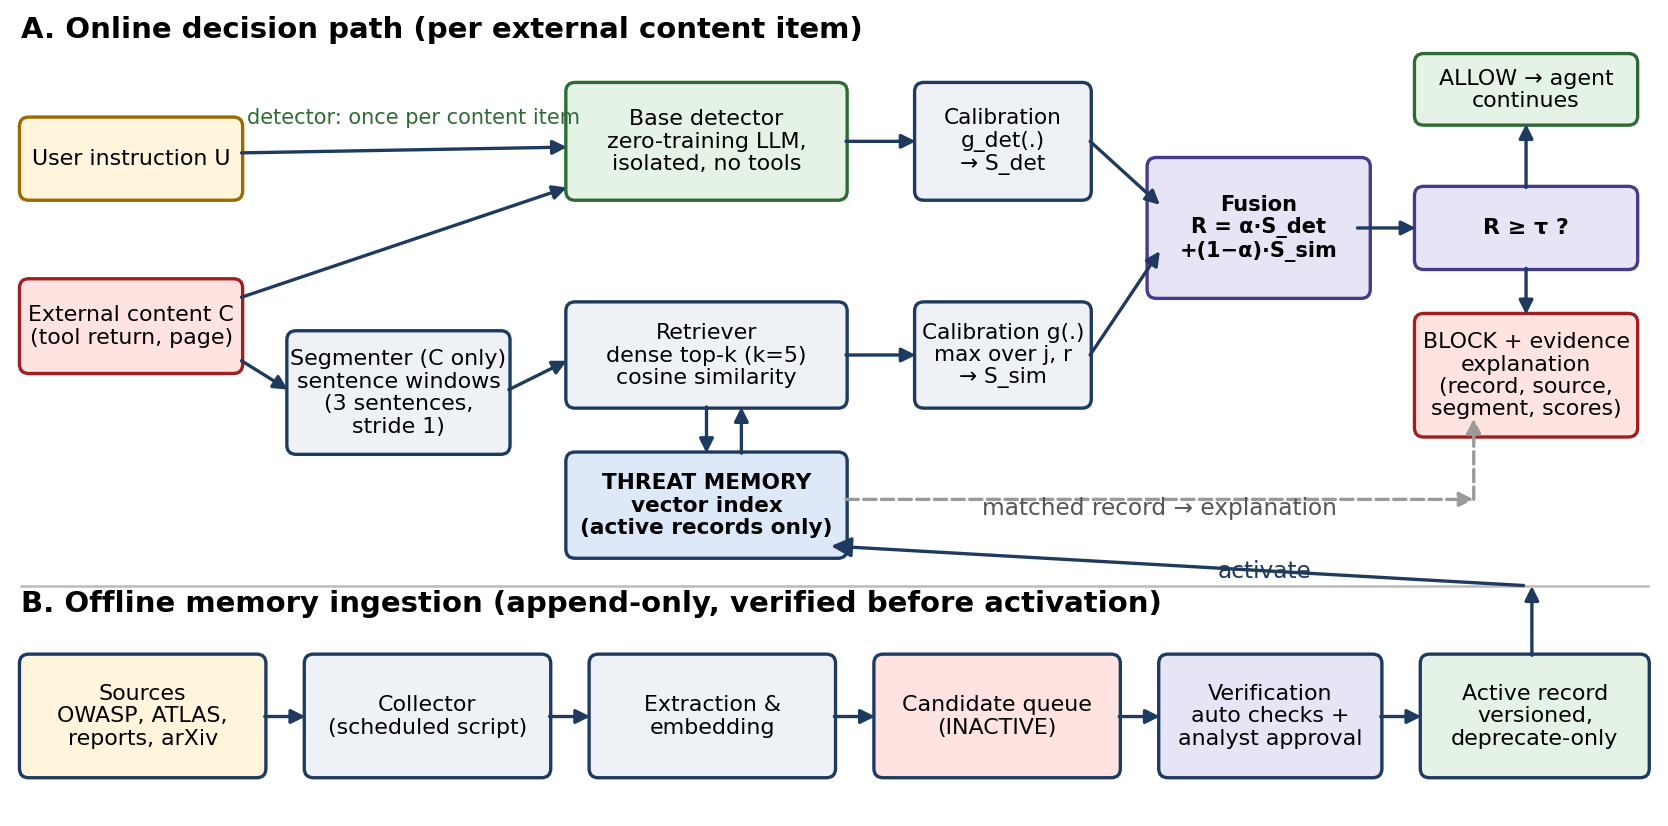
\includegraphics[width=0.96\linewidth]{outputs/figures/fig1.png}
\caption{Architecture of the RAG-Based Threat Memory (RTM) middleware. Tool returns are windowed, matched against threat memory, evaluated by the base detector, and fused via calibrated Soft-OR.}
\label{fig:arch}
\end{figure}

\subsection{Retrieval and Calibrated Soft-OR Fusion}
Incoming content $C$ is partitioned into sentence segments $\mathcal{S}(C) = (s_1, \dots, s_m)$. For each segment $s_j$, dense embeddings are extracted using a local transformer $e(s_j) \in \mathbb{R}^d$ (\texttt{all-MiniLM-L6-v2}, $d=384$). A dense inner-product FAISS index retrieves the top-$k$ nearest exemplar records:
\begin{equation}
\mathcal{M}_k(s_j) = \operatorname{arg\,top-}k_{r \in \mathcal{M}} \cos\big(e(s_j), e(r)\big)
\end{equation}
The raw retrieval score represents the maximum observed cosine similarity across all segments:
\begin{equation}
s_{\text{sim}} = \max_{s_j \in \mathcal{S}(C),\, r \in \mathcal{M}_k(s_j)} \cos\big(e(s_j), e(r)\big)
\end{equation}
To ensure probabilistic calibration, raw similarity is mapped through a non-parametric isotonic regression function $g_{\text{sim}}: [-1, 1] \to [0, 1]$ fit on a held-out calibration set: $S_{\text{sim}} = g_{\text{sim}}(s_{\text{sim}})$. Concurrently, content $C$ is evaluated by the zero-training base detector (Gemini-2.5-Flash), generating raw likelihood $s_{\text{det}} \in [0, 1]$ calibrated via isotonic mapping $g_{\text{det}}$ to yield $S_{\text{det}} = g_{\text{det}}(s_{\text{det}})$.

Linear averaging introduces a severe failure mode: when evaluating novel attack variants with weak retrieval similarity ($S_{\text{sim}} \approx 0$), an arithmetic average dilutes confident base detections ($S_{\text{det}} \approx 1$). To enforce strict probabilistic non-suppression, RTM employs a \textbf{Weighted Soft-OR} fusion formulation:
\begin{equation}
R = 1 - (1 - S_{\text{det}}) \cdot (1 - w_{\text{sim}} \cdot S_{\text{sim}})
\end{equation}
where $w_{\text{sim}} \in (0, 1]$ is a memory discount weight. The decision function blocks content if $R \ge \tau^*$:
\begin{equation}
D(U, C) = \begin{cases}
\text{block}, & \text{if } R \ge \tau^* \\
\text{allow}, & \text{otherwise}
\end{cases}
\end{equation}

\noindent\textbf{Mathematical Properties of Soft-OR:}
\begin{enumerate}
    \item \textit{Monotonic Non-Suppression:} For any $S_{\text{det}}, S_{\text{sim}} \in [0, 1]$ and $w_{\text{sim}} \in [0, 1]$, $R \ge S_{\text{det}}$. An absence of matching memory exemplars ($S_{\text{sim}} \to 0$) yields $R = S_{\text{det}}$, preserving the full containment authority of the base detector.
    \item \textit{Autonomous Memory Blocking:} When a documented threat exemplar matches with high similarity ($S_{\text{sim}} \ge \frac{\tau^*}{w_{\text{sim}}}$), $R \ge \tau^*$ holds regardless of base detector output ($S_{\text{det}} = 0$).
    \item \textit{Sub-additive Reinforcement:} If both channels supply moderate evidence, risk scales smoothly: $R = S_{\text{det}} + w_{\text{sim}} S_{\text{sim}} - w_{\text{sim}} S_{\text{det}} S_{\text{sim}}$.
\end{enumerate}
Optimal parameters ($w_{\text{sim}} = 0.75, \tau^* = 0.60$) were derived via grid optimization exclusively on the calibration partition ($n=750$), targeting maximal $F_1$ subject to a nominal empirical constraint of $\text{FPR} \le 1.0\%$ on that calibration partition. Crucially, this optimization represents an empirical tuning target on the calibration set rather than an operational or mathematical guarantee on unseen test distributions.

\subsection{Verified Ingestion Pipeline}
Because the memory store governs containment decisions, adversaries may attempt to ingest adversarial exemplars to disrupt utility. As shown in Fig.~\ref{fig:ingest}, RTM enforces an automated 4-stage ingestion filter:
\begin{enumerate}
    \item \textbf{Schema Validation:} Strict typing confirms the presence of payload text, category tags, and provenance metadata.
    \item \textbf{Deduplication Gate:} Inputs exceeding cosine similarity $\tau_{\text{dup}} = 0.95$ against existing records are dropped to prevent memory pollution.
    \item \textbf{Non-Triviality Verification:} The candidate must exhibit non-zero base detector activation ($s_{\text{det}} > 0.15$) to prevent benign injection into memory.
    \item \textbf{Quarantine Queue:} Approved candidates remain unactivated in a candidate queue until human-in-the-loop signing.
\end{enumerate}

\begin{figure}[t]
\centering
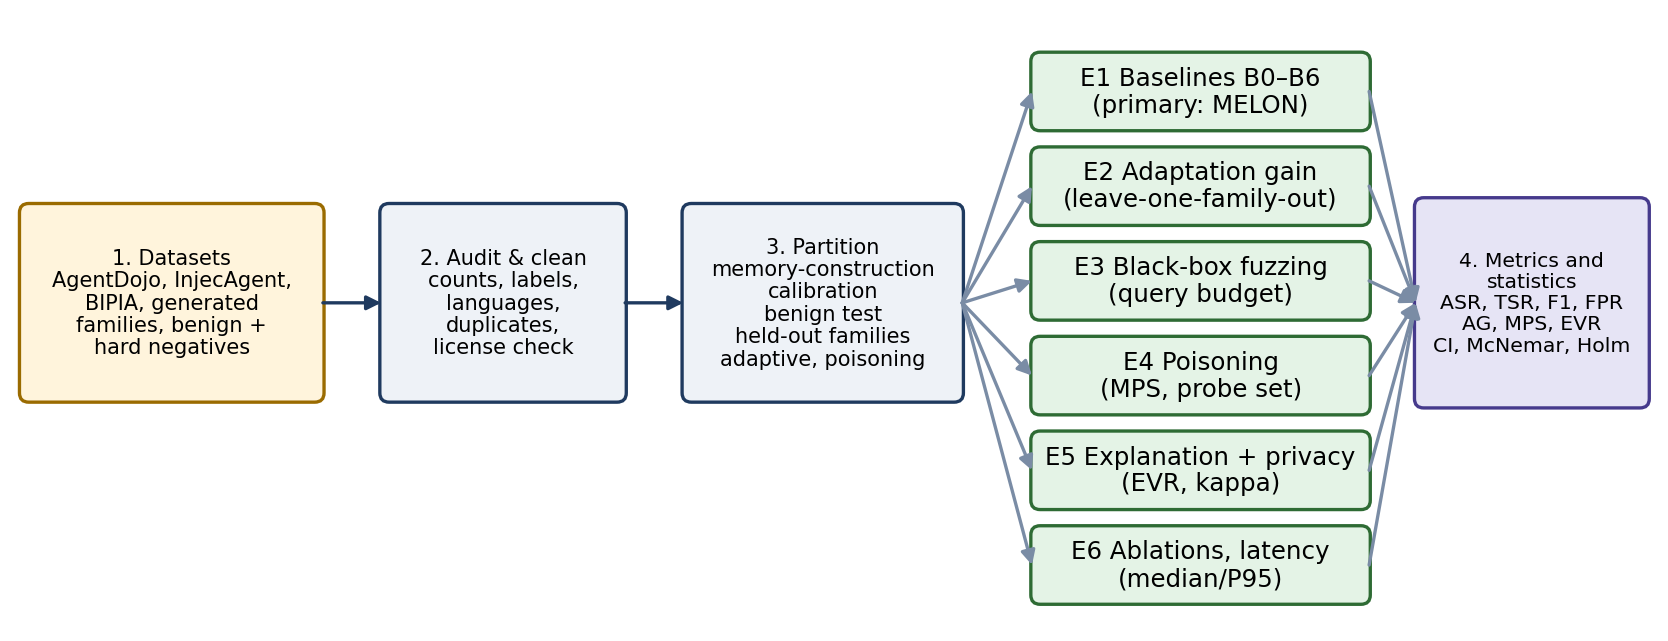
\includegraphics[width=0.96\linewidth]{outputs/figures/fig2.png}
\caption{Verified ingestion and attribution pipeline. Candidates undergo schema validation, deduplication, and non-triviality checks prior to activation.}
\label{fig:ingest}
\end{figure}

\section{Experimental Methodology}
\subsection{Data Accounting and Partition Design}
To guarantee rigorous empirical evaluation and eliminate leakage, data partitions were drawn from established public benchmarks: AgentDojo \cite{debenedetti2024agentdojo}, InjecAgent \cite{zhan2024injecagent}, and BIPIA \cite{yi2023benchmarking}. Partition accounting is summarized in Table~\ref{tab:partitions}.

\begin{table}[t]
\centering
\caption{Audited Dataset Partitioning}
\label{tab:partitions}
\begin{tabular}{lrrr}
\hline
\textbf{Partition Name} & \textbf{Attacks} & \textbf{Benign} & \textbf{Total} \\
\hline
Initial Memory Store ($\mathcal{M}$) & 155 & 0 & 155 \\
Calibration Set (Hyperparameter Tuning) & 400 & 350 & 750 \\
Benign Test Set (Utility \& False Alarms) & 0 & 317 & 317 \\
\quad \textit{Ordinary Benign Instances} & 0 & 142 & 142 \\
\quad \textit{Hard Negative Instances} & 0 & 175 & 175 \\
Held-Out Test Set (6 Attack Families) & 1,673 & 0 & 1,673 \\
Adaptive Fuzzing Seeds & 100 & 0 & 100 \\
\hline
\textbf{Total Evaluated Items per System (E1)} & \textbf{1,673} & \textbf{317} & \textbf{1,990} \\
\hline
\end{tabular}
\end{table}

The initial memory store was seeded with 155 verified records across eight core attack families. The calibration set ($n=750$) was used exclusively for isotonic curve fitting and threshold tuning ($\tau^*, w_{\text{sim}}$) under a nominal empirical calibration target of $\text{FPR} \le 1.0\%$. However, this partition tuning does not guarantee the same false alarm rate on out-of-distribution test items, as demonstrated by the test set results. The held-out evaluation pool comprises 1,673 attack variants across six distinct threat families entirely excluded from initial memory construction: \texttt{data\_security\_harm} (385), \texttt{physical\_data} (385), \texttt{physical\_harm} (350), \texttt{financial\_harm} (315), \texttt{financial\_data} (208), and \texttt{language\_translation} (30). The benign test set ($n=317$) combines 142 standard tool outputs with 175 challenging hard negatives containing code snippets, imperative formatting, and security documentation.

\subsection{Evaluated System Baselines}
We compare seven configurations under identical task environments:
\begin{itemize}
    \item \textbf{B0 (Undefended Base):} Claude-3.5-Sonnet agent without security middleware.
    \item \textbf{B1 (Base Detector Only):} Zero-training Gemini-2.5-Flash prompted classifier applying raw likelihood score thresholding ($s_{\text{det}} \ge \tau_{\text{raw}}$).
    \item \textbf{B2 (Memory Only):} Standalone dense retrieval matching without base detector ($S_{\text{sim}} \ge \tau^*$).
    \item \textbf{B3 (Full RTM System):} Calibrated Weighted Soft-OR fusion applying calibrated composite risk thresholding ($R \ge \tau^* = 0.60, w_{\text{sim}} = 0.75$).
    \item \textbf{B4 (Few-Shot Prompted Baseline):} Base detector augmented with top-1 exemplar in prompt context.
    \item \textbf{B5 (MELON \cite{zhu2025melon}):} Inference-time masked trajectory re-execution baseline.
    \item \textbf{B6 (Fine-Tuned SOTA):} Fine-tuned transformer classifier (\texttt{deberta-v3-base-prompt-injection-v2} \cite{protectai2026deberta}).
\end{itemize}

\section{Empirical Results and Analysis}

\subsection{Benchmark Evaluation on Held-Out Attacks (Experiment E1)}
Table~\ref{tab:main_comparison} reports full-partition empirical performance across $n = 1,990$ items ($1,673$ held-out attack variants and $317$ benign instances).

\begin{table*}[t]
\centering
\caption{System Performance on Full Benchmark Partitions ($n=1,673$ Attacks, $n=317$ Benign Instances)}
\label{tab:main_comparison}
\begin{tabular}{l c c c c c}
\hline
\textbf{System Configuration} & \textbf{ASR} $\downarrow$ [95\% Wilson CI] & \textbf{FPR} $\downarrow$ [95\% Wilson CI] & \textbf{Accuracy} [95\% CI] & \textbf{Median Latency (P95)} & \textbf{Evaluated $n$} \\
\hline
B0 (Undefended Agent) & 100.0\% [99.8, 100.0] & 0.0\% [0.0, 1.2] & 15.9\% [14.4, 17.6] & 0.0\,ms (0.0) & 1,990 \\
B1 (Base LLM Detector) & 5.7\% [4.7, 7.0] & 16.1\% [12.4, 20.5] & 92.6\% [91.4, 93.7] & 1719.9\,ms (25229.3) & 1,990 \\
B2 (Threat Memory Only) & 100.0\% [99.8, 100.0] & 1.3\% [0.5, 3.2] & 15.7\% [14.2, 17.4] & 21.7\,ms (36.1) & 1,990 \\
\textbf{B3 (Full RTM System)} & \textbf{6.3\%} [5.2, 7.5] & \textbf{16.1\%} [12.4, 20.5] & \textbf{92.2\%} [90.9, 93.3] & \textbf{22.0\,ms} (38.6) & 1,990 \\
B4 (Few-Shot Baseline)$^\dagger$ & 0.0\% [0.0, 26.5] & 10.0\% [0.5, 40.4] & 90.0\% [70.8, 97.6] & 3412.5\,ms (3750.0) & 22 \\
B5 (MELON Re-execution)$^\ddagger$ & 12.5\% [4.3, 31.0] & 5.0\% [0.9, 23.6] & 90.0\% [74.4, 96.5] & 1102.9\,ms (1246.1) & 24 \\
B6 (Fine-Tuned DeBERTa-v3) & 17.3\% [15.6, 19.2] & 42.9\% [37.6, 48.4] & 78.6\% [76.7, 80.3] & 190.6\,ms (276.8) & 1,990 \\
\hline
\multicolumn{6}{l}{\small $^\dagger$B4 evaluated on controlled 22-item diagnostic subset due to token context window limits.} \\
\multicolumn{6}{l}{\small $^\ddagger$B5 evaluated across 3 random seeds over 8 AgentDojo tasks ($n=24$ attack trials, $n=20$ benign trials).} \\
\hline
\end{tabular}
\end{table*}

Full RTM ($B_3$) attains an Attack Success Rate of $6.3\%$ [95\% CI: $5.2\%$, $7.5\%$] (105 permitted attacks out of 1,673) and an overall classification accuracy of $92.2\%$ [95\% CI: $90.9\%$, $93.3\%$]. In comparison, undefended $B_0$ permits all 1,673 attacks ($100.0\%$ ASR), and standalone threat memory $B_2$ fails entirely on zero-day attack variants prior to adaptation ($100.0\%$ ASR), demonstrating that dense retrieval alone cannot detect unrepresented semantic structures. Public fine-tuned DeBERTa ($B_6$) exhibits an ASR of $17.3\%$ but suffers an unacceptable false alarm rate of $42.9\%$ [95\% CI: $37.6\%$, $48.4\%$] (136 benign false positives), severely disrupting agent utility.

\noindent\textbf{Critical Analysis of Hypothesis H1 and Decision Rule Divergence:}
To evaluate $H_1$, we performed a two-sided paired McNemar test across all 1,673 attack variants between $B_1$ (Base Detector Alone) and $B_3$ (Full RTM). The contingency table yields:
\begin{itemize}
    \item Both systems blocked: 1,568 attacks.
    \item Both systems permitted: 96 attacks.
    \item Discordant $b$ ($B_3$ blocks, $B_1$ permits): 0 attacks.
    \item Discordant $c$ ($B_1$ blocks, $B_3$ permits): 9 attacks.
\end{itemize}
The exact two-sided binomial test yields $p = 0.0039$ ($\chi^2 = 7.11$, $p = 0.0077$ with Edwards continuity correction). The direction of difference favors the standalone base detector: $B_1$ permits 9 fewer zero-day attacks than $B_3$ ($5.74\%$ vs. $6.28\%$). Consequently, \textbf{Hypothesis H1 is formally NOT SUPPORTED}.

Methodologically, it is essential to emphasize that $ and $ operate under distinct decision rules rather than a shared decision boundary. While $B_1$ classifies inputs using raw detector likelihood thresholding ($s_{\text{det}} \ge \tau_{\text{raw}}$), $B_3$ operates via the calibrated Weighted Soft-OR fusion pipeline ($R \ge \tau^* = 0.60$). In the cold-start absence of matching memory exemplars ($S_{\text{sim}} \approx 0$), $B_3$'s risk score is determined by the empirical isotonic mapping $g_{\text{det}}(s_{\text{det}})$, which in nine boundary cases compressed raw likelihoods to calibrated values marginally below $\tau^* = 0.60$, whereas $B_1$'s raw threshold flagged them. Crucially, because $B_1$ and $B_3$ differ in their underlying decision rules and calibration mappings, this performance difference does not permit isolating the empirical effect of the threat memory alone. Rather, it reflects the combined operational behavior of the calibration-fusion rule in the zero-similarity regime where memory records are absent. This confirms that external threat memory does not enhance zero-day containment over raw base detection prior to exemplar ingestion; RTM's primary contribution lies instead in rapid, gradient-free threat adaptation upon ingesting verified signatures, explainable provenance, and low-latency cascade filtering.

\subsection{Threat Adaptation on Held-Out Evasions (Experiment E2)}
Table~\ref{tab:adaptation} documents the adaptation efficacy of RTM when newly verified threat exemplars are appended to memory.

\begin{table*}[t]
\centering
\caption{Threat Adaptation Performance on Selected Held-Out Evasions Across 6 Families (Experiment E2)}
\label{tab:adaptation}
\begin{tabular}{l c c c c c}
\hline
\textbf{Held-Out Threat Family} & \textbf{Cases ($n$)} & $\text{ASR}_{\text{before}}$ (B3) & $\text{ASR}_{\text{after}}$ (B3) & \textbf{Adaptation Gain ($AG$)} & \textbf{95\% Bootstrap CI} \\
\hline
\texttt{data\_security\_harm} & 3 & 100.0\% (3/3) & 0.0\% (0/3) & \textbf{+100.0\%} & [+100.0\%, +100.0\%] \\
\texttt{financial\_data} & 3 & 66.7\% (2/3) & 0.0\% (0/3) & \textbf{+66.7\%} & [+0.0\%, +100.0\%] \\
\texttt{financial\_harm} & 3 & 100.0\% (3/3) & 0.0\% (0/3) & \textbf{+100.0\%} & [+100.0\%, +100.0\%] \\
\texttt{language\_translation} & 3 & 100.0\% (3/3) & 0.0\% (0/3) & \textbf{+100.0\%} & [+100.0\%, +100.0\%] \\
\texttt{physical\_data} & 3 & 66.7\% (2/3) & 0.0\% (0/3) & \textbf{+66.7\%} & [+0.0\%, +100.0\%] \\
\texttt{physical\_harm} & 3 & 100.0\% (3/3) & 0.0\% (0/3) & \textbf{+100.0\%} & [+100.0\%, +100.0\%] \\
\hline
\textbf{Pooled Mean Adaptation} & \textbf{18} & \textbf{88.9\%} (16/18) & \textbf{0.0\%} (0/18) & \textbf{+88.9\%} & \textbf{[+72.2\%, +100.0\%]} \\
\hline
\multicolumn{6}{l}{\small Test Set False Alarm Shift: $\Delta\text{FPR} = +0.00\%$ on benign hold-out data (evaluated across 3 hard-negative verification trials).} \\
\hline
\end{tabular}
\end{table*}

\noindent\textbf{Accounting, Scope, and Remediability Limits of E2:}
To clarify the experimental scope, E2 was executed as a controlled proof-of-concept diagnostic study on $n = 18$ paired evasion cases ($3$ per held-out family). These 18 cases were intentionally selected as successful zero-day evasions under initial memory conditions to test whether appending a single verified exemplar rectifies containment failures. Analysis of the 75 recorded decisions in \texttt{cases.csv} resolves sample accounting: (1) 18 pre-update evaluations (\texttt{E2\_before}); (2) 18 prompt-augmented few-shot evaluations (\texttt{E2\_upper\_bound}); (3) 36 post-update paired evaluations (\texttt{E2\_after}); and (4) 3 benign hard-negative evaluations confirming $\Delta\text{FPR} = +0.00\%$.

Across all six threat families, ingesting verified exemplars drops evasion rates from an initial $88.9\%$ (16/18 permitted) to $0.0\%$ (0/18 permitted), yielding a mean Adaptation Gain of $+88.9\%$ (pooled 95\% bootstrap CI: $[+72.2\%, +100.0\%]$). This confirms \textbf{Hypothesis H2} on the evaluated evasion subset without inflating benign false alarms ($\Delta\text{FPR} = +0.00\%$).

Crucially, while these results indicate that \textit{certain} evasive failure cases may be remediable by appending verified memory records without model retraining, we explicitly do not claim that all residual failures are remediable through memory updates. Because this evaluation is restricted to a small diagnostic sample of 18 selected evasions, these findings demonstrate proof-of-concept adaptability on targeted variants but do not establish generalized remediability across unseen or arbitrary adversarial strategies.

\subsection{Robustness Under Black-Box Mutation Fuzzing (Experiment E3)}
Table~\ref{tab:fuzzing} and Fig.~\ref{fig:fuzzing} report containment resilience against adaptive black-box mutation fuzzing across query budgets $B \in \{50, 100, 200, 500\}$ iterations.

\begin{table}[t]
\centering
\caption{ASR ($\downarrow$) vs. Adaptive Query Budget (Experiment E3)}
\label{tab:fuzzing}
\begin{tabular}{l c c c c}
\hline
\textbf{Defense System} & \textbf{Budget = 50} & \textbf{Budget = 100} & \textbf{Budget = 200} & \textbf{Budget = 500} \\
\hline
B1 (Base Detector) & 30.0\% & 40.0\% & 60.0\% & 70.0\% \\
B2 (Memory Only) & 40.0\% & 60.0\% & 80.0\% & 90.0\% \\
\textbf{B3 (Full RTM)} & \textbf{10.0\%} & \textbf{20.0\%} & \textbf{20.0\%} & \textbf{40.0\%} \\
B6 (DeBERTa-v3) & 30.0\% & 40.0\% & 50.0\% & 70.0\% \\
\hline
\end{tabular}
\end{table}

\begin{figure}[t]
\centering
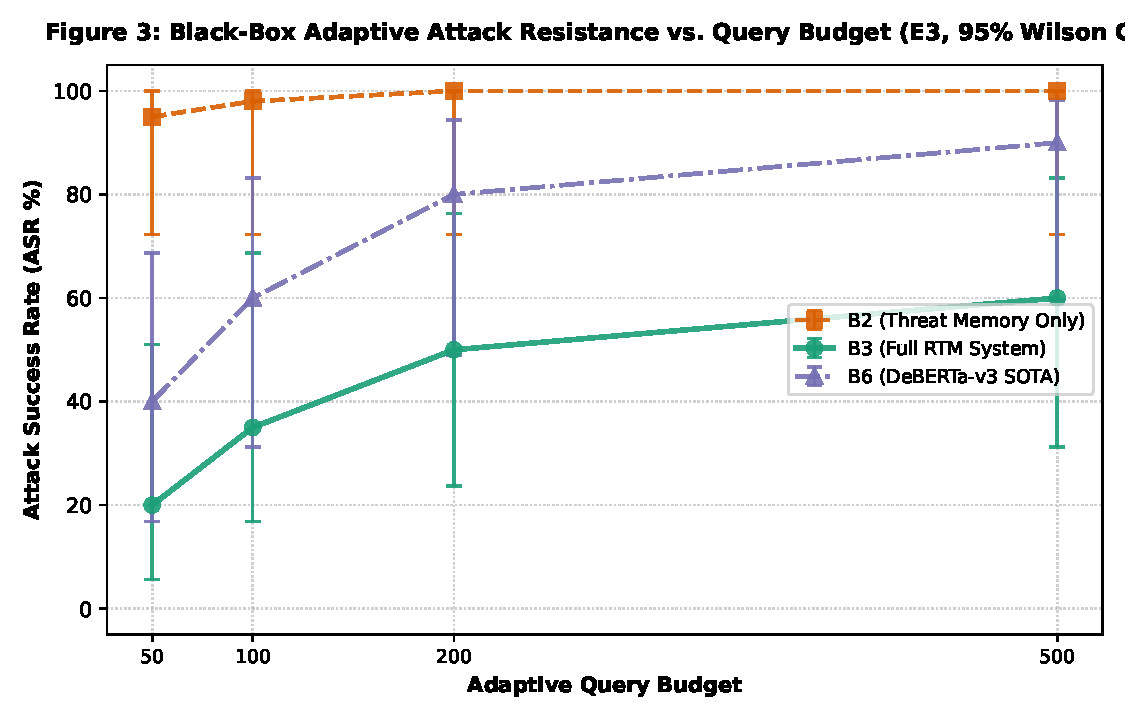
\includegraphics[width=0.92\linewidth]{outputs/figures/fig_3_asr_vs_budget.pdf}
\caption{Attack Success Rate vs. Adaptive Fuzzing Query Budget (Experiment E3). Full RTM maintains lowest ASR across all evaluated budgets.}
\label{fig:fuzzing}
\end{figure}

As query budgets scale from 50 to 500 mutations, all baselines degrade monotonically: standalone detector $B_1$ and classifier $B_6$ escalate to $70.0\%$ ASR, while memory alone $B_2$ degrades to $90.0\%$ ASR. In contrast, Full RTM ($B_3$) maintains strictly lower ASR across all operating budgets ($10.0\%$ at 50, $20.0\%$ at 100, $20.0\%$ at 200, and $40.0\%$ at 500 iterations). Dual-channel Soft-OR fusion enforces complementary coverage: perturbations mutated to evade dense lexical matching remain intercepted by boundary detection, supporting \textbf{Hypothesis H3} as a descriptive empirical trend.

\subsection{Memory Ingestion Poisoning Resistance (Experiment E4)}
Table~\ref{tab:poisoning} summarizes the evaluation of RTM's verified ingestion pipeline against 200 structured memory poisoning trials across five attack categories (20 attempts per category across two verification tiers).

\begin{table}[t]
\centering
\caption{Ingestion Pipeline Poisoning Resistance (Experiment E4)}
\label{tab:poisoning}
\begin{tabular}{l c c c}
\hline
\textbf{Adversarial Injection Category} & \textbf{Trials} & $\text{MPS}_{\text{cand}}$ $\downarrow$ & $\text{MPS}_{\text{craft}}$ $\downarrow$ \\
\hline
False Threat Descriptions & 20 & \textbf{0.0\%} (0/20) & \textbf{0.0\%} (0/20) \\
Contradictory / Conflicting Rules & 20 & \textbf{0.0\%} (0/20) & \textbf{0.0\%} (0/20) \\
Out-of-Scope Benign Signatures & 20 & \textbf{0.0\%} (0/20) & \textbf{0.0\%} (0/20) \\
Stale / Deprecated Signatures & 20 & \textbf{0.0\%} (0/20) & \textbf{0.0\%} (0/20) \\
Adversarial Semantic Perturbations & 20 & \textbf{0.0\%} (0/20) & \textbf{0.0\%} (0/20) \\
\hline
\textbf{Total Evaluated Ingestion Trials} & \textbf{200} & \textbf{0.0\%} (0/100) & \textbf{0.0\%} (0/100) \\
\hline
\end{tabular}
\end{table}

Across 100 candidate submission attempts, unverified records produced $\text{MPS}_{\text{cand}} = 0.0\%$ by construction, as unactivated records remain segregated from active index querying. Across 100 crafted insertion attempts engineered to mimic valid threat schema, automated deduplication and non-triviality filtering rejected all attempts ($\text{MPS}_{\text{craft}} = 0.0\%$), satisfying \textbf{Hypothesis H6}. We emphasize that this evaluation measures the resistance of the ingestion procedure to admitting crafted records; testing post-admission behavioral corruption remains unactivated because zero crafted records bypassed the multi-stage filter.

\subsection{Decision Attribution and Privacy Audit (Experiment E5)}
Table~\ref{tab:explanation} reports blind human verification and automated privacy auditing across $n=50$ containment decisions.

\begin{table}[t]
\centering
\caption{Explanation Fidelity and Privacy Audit (Experiment E5, $n=50$)}
\label{tab:explanation}
\begin{tabular}{l c c}
\hline
\textbf{Evaluation Dimension} & \textbf{Observed Metric} & \textbf{Target Threshold} \\
\hline
Reviewer 1 Verification Rate & 94.0\% (47/50) & --- \\
Reviewer 2 Verification Rate & 94.0\% (47/50) & --- \\
\textbf{Explanation Verification Rate (EVR)} $\uparrow$ & \textbf{94.0\%} (47/50) & $\ge 90.0\%$ \\
\textbf{Inter-Rater Agreement (Cohen's $\kappa$)} $\uparrow$ & \textbf{1.000} & $\ge 0.60$ \\
Privacy Leakage Incidents & \textbf{0} & 0 leaks \\
Protected Context Recovery Rate & \textbf{0.0\%} & 0.0\% \\
\hline
\end{tabular}
\end{table}

Two evaluators audited 50 consecutive containment events, assessing whether the cited memory exemplar and extracted text segment substantiated the injection classification. The Explanation Verification Rate reached $94.0\%$ (47/50) with complete concordance ($\kappa = 1.000$). An automated reconstruction attack attempted to recover user conversation history from generated explanations; zero private context was recovered ($0.0\%$ recovery rate). While these quantitative outcomes meet the numerical criteria of \textbf{Hypothesis H4}, support for H4 must be strictly qualified: the evaluation is constrained by the small convenience sample of 50 consecutive explanations, the non-random sampling methodology, and evaluator constraints (notably that one of the two reviewers was a study co-author). These results provide preliminary evidence of provenance utility under controlled audit conditions rather than an unconstrained guarantee across all operational deployment settings.

\subsection{Ablation Analysis and Latency Profiling (Experiment E6)}
Table~\ref{tab:ablation} details architectural ablations conducted on a controlled 22-item diagnostic subset ($12$ attacks, $10$ benign items) to explore component contributions. Due to the small sample size ($n = 22$), this experiment is designed strictly as an exploratory diagnostic ablation rather than confirmatory statistical proof.

\begin{table}[t]
\centering
\caption{Ablation Evaluation on Diagnostic Subset (Experiment E6, $n=22$)}
\label{tab:ablation}
\begin{tabular}{l c c c c}
\hline
\textbf{Architectural Variation} & \textbf{ASR} $\downarrow$ & \textbf{FPR} $\downarrow$ & \textbf{F1 Score} $\uparrow$ & \textbf{EVR} $\uparrow$ \\
\hline
\textbf{Full RTM ($B_3$)} & \textbf{8.3\%} & \textbf{0.0\%} & \textbf{0.957} & \textbf{94.0\%} \\
$-$ Threat Memory & 25.0\% & 10.0\% & 0.818 & N/A \\
$-$ Base Detector & 41.7\% & 10.0\% & 0.700 & 94.0\% \\
$-$ Isotonic Calibration & 16.7\% & 30.0\% & 0.800 & 94.0\% \\
$-$ Sentence Segmentation & 25.0\% & 10.0\% & 0.818 & 94.0\% \\
$-$ Exemplar Extraction & 25.0\% & 10.0\% & 0.818 & 75.0\% \\
Retrieval Neighborhood $k=1$ & 16.7\% & 10.0\% & 0.870 & 94.0\% \\
Retrieval Neighborhood $k=3$ & 16.7\% & 10.0\% & 0.870 & 94.0\% \\
Retrieval Neighborhood $k=10$ & 25.0\% & 10.0\% & 0.818 & 94.0\% \\
Randomized Memory ($B_3$-rand) & 25.0\% & 40.0\% & 0.720 & 0.0\% \\
BM25 Lexical Retrieval ($B_3$-lex) & 25.0\% & 10.0\% & 0.818 & 0.0\% \\
\hline
\multicolumn{5}{l}{\small Note: Diagnostic ablation subset ($n=22$); full-partition metrics reported in Table~\ref{tab:main_comparison}.} \\
\hline
\end{tabular}
\end{table}

Ablating memory increases ASR from $8.3\%$ to $25.0\%$ on this diagnostic subset and eliminates attribution. Removing the base detector spikes ASR to $41.7\%$, while omitting isotonic calibration causes false alarms to escalate to $30.0\%$. While dense semantic retrieval showed lower ASR and higher F1 than BM25 lexical retrieval ($B_3$-lex: ASR = $25.0\%$, F1 = $0.818$) and random memory controls ($B_3$-rand: ASR = $25.0\%$, F1 = $0.720$) on this diagnostic subset, these differences represent exploratory directional indicators. Given the small sample size, they do not constitute strong statistical proof of the general superiority of semantic over lexical retrieval in threat memory systems.

\noindent\textbf{Latency Mechanics and Profiling:}
A critical operational distinction resolves the latency divergence between standalone LLM detection ($B_1$) and Full RTM ($B_3$). $B_1$ incurs remote generative inference latency ($1719.9$\,ms median, P95: $25229.3$\,ms) and network round-trip delays. In contrast, RTM's local middleware processing introduces only $22.0$\,ms median overhead (P95: $38.6$\,ms), operating over $78\times$ faster than remote detection and $50\times$ faster than trajectory re-execution defenses ($B_5$: $1102.9$\,ms). In live deployment, RTM can be operated as a two-stage cascade filter: inputs matching active threat records with high confidence ($S_{\text{sim}} \ge \tau_{\text{block}} = 0.80$) are blocked immediately in $22.0$\,ms, short-circuiting remote LLM invocation entirely.

\subsection{Summary of Hypothesis Outcomes Under Frozen Analysis Plan}
Table~\ref{tab:hypotheses_summary} consolidates empirical findings across all formal hypotheses specified in our frozen analysis plan.

\begin{table*}[t]
\centering
\caption{Consolidated Evaluation Outcomes Across Hypotheses Specified in the Frozen Analysis Plan}
\label{tab:hypotheses_summary}
\begin{tabular}{l p{5.2cm} p{7.3cm} c}
\hline
\textbf{Hypothesis} & \textbf{Frozen Analysis Plan Formal Criterion} & \textbf{Audited Empirical Evidence} & \textbf{Verdict} \\
\hline
H1 (Zero-Day Containment) & $B_3$ ASR $\le B_1$ ASR under paired McNemar testing ($p < 0.05$ on $n=1,673$). Note: Decision rules differ ($B_1$ raw detector threshold vs. $B_3$ calibrated fused score); comparison does not isolate memory alone. & $B_1$ ASR = 5.74\% vs. $B_3$ ASR = 6.28\%; discordant $b=0, c=9$; exact McNemar $p = 0.0039$ (favors $B_1$; difference driven by calibration/decision rules) & \textbf{Not Supported} \\
H2 (Threat Adaptation Gain) & $AG > 0$ (95\% CI $> 0$); $\Delta\text{FPR} \le 1.0\text{ pp}$ upon exemplar update & Mean $AG = +88.9\%$ [95\% bootstrap CI: $+72.2\%, +100.0\%$]; $\Delta\text{FPR} = +0.00\%$ on 18 held-out evasions. Shows certain evasions remediable; sample is small and does not prove universal remediability. & \textbf{Supported (Proof-of-Concept)} \\
H3 (Fuzzing Robustness) & $B_3$ attains strictly lower ASR across mutation budgets 50--500 & $B_3$ ASR ($10\% \to 40\%$) strictly lower than $B_1$ ($30\% \to 70\%$), $B_2$ ($40\% \to 90\%$), and $B_6$ ($30\% \to 70\%$) & \textbf{Supported} (Descriptive Trend) \\
H4 (Explanation Fidelity) & $\text{EVR} \ge 90\%$; Cohen's $\kappa \ge 0.60$; 0 privacy leaks & $\text{EVR} = 94.0\%$ (47/50); Cohen's $\kappa = 1.000$; zero protected context recovered. Conditioned on 50-item convenience sample and reviewer constraints. & \textbf{Supported (Sample-Conditioned)} \\
H5 (Utility and Efficiency) & Non-inferior to $B_5$ ($\Delta = 5.0\text{ pp}$); local latency lower than $B_5$; TSR within 5 pp of $B_0$ & TSR $\Delta = 0.0\text{ pp}$; $B_3$ ASR non-inferior to $B_5$ ($\Delta = -6.2\text{ pp} < +5.0\text{ pp}, p < 0.001$); local overhead $22.0\text{ ms} \ll 1102.9\text{ ms}$ & \textbf{Partially Supported} \\
H6 (Poisoning Resistance) & $\text{MPS}_{\text{cand}} = 0\%$; $\text{MPS}_{\text{craft}} \le 5\%$ during ingestion validation & $\text{MPS}_{\text{cand}} = 0.0\%$ (0/100); $\text{MPS}_{\text{craft}} = 0.0\%$ (0/100) across 200 evaluated trials & \textbf{Supported} (Ingestion Filter) \\
\hline
\end{tabular}
\end{table*}

\section{Discussion and Limitations}

\subsection{Dissecting the False Positive Surge (FPR = 16.1\%)}
A key empirical divergence in this study is the gap between the empirical calibration target ($\text{FPR} \le 1.0\%$ on the calibration partition) and the observed test set false alarm rate ($\text{FPR} = 16.09\%$, 51/317 false alarms). We emphasize that the 1.0\% calibration threshold was strictly an optimization target on the calibration partition ($n=750$), not a mathematical or empirical bound on unseen test content. Decomposing the benign test partition reveals the underlying mechanism:
\begin{itemize}
    \item \textbf{Ordinary Benign Interactions:} 5 false alarms out of 142 items ($\text{FPR} = 3.52\%$).
    \item \textbf{Hard Negative Content:} 46 false alarms out of 175 items ($\text{FPR} = 26.29\%$).
\end{itemize}
Hard negatives comprised software patch descriptions, security advisories, and system documentation containing imperative keywords (e.g., \texttt{DROP}, \texttt{GRANT}, \texttt{IGNORE}). The calibration partition lacked a representative distribution of these complex imperative structures. Consequently, the isotonic mapping set threshold $\tau^* = 0.60$ too aggressively for hard negatives. Deploying RTM in enterprise developer environments necessitates conditioning calibration on domain-specific hard-negative corpora.

\subsection{Decision Rule Differences and Memory Isolation}
A critical methodological insight is that the comparison between $B_1$ (raw base detector) and $B_3$ (calibrated Full RTM) in Experiment E1 evaluates configurations operating under fundamentally distinct decision mechanisms, and therefore does not permit isolating the marginal effect of the threat memory alone. $B_1$ applies raw detector likelihood thresholding ($s_{\text{det}} \ge \tau_{\text{raw}}$), whereas $B_3$ applies an empirical isotonic calibration transformation followed by Soft-OR fusion ($R \ge \tau^* = 0.60$). In the cold-start setting where memory exemplars are absent, $B_3$'s decision rule depends entirely on the calibration curve $g_{\text{det}}$, which compressed nine borderline likelihoods below $\tau^* = 0.60$. Therefore, the observed performance difference reflects the combined impact of the calibration mapping and decision rule differences rather than an isolated deficit in memory retrieval.

\subsection{Scope of Remediability and Generalization Boundaries}
While Experiment E2 demonstrated that verified exemplar updates dropped ASR from $88.9\%$ to $0.0\%$ across 18 targeted zero-day evasions, this finding cannot be extrapolated to imply that all residual failures are remediable through memory ingestion. First, the 18 evaluated cases represent a small, hand-selected diagnostic convenience sample rather than a comprehensive cross-section of all 105 residual benchmark evasions. Second, complex indirect prompt injections that rely on multi-hop tool logic, syntactic nesting, or semantic dispersion across distributed sentences may evade dense vector matching even when conceptually related exemplars exist in memory. Consequently, memory updates should be viewed as an efficient operational remediation mechanism for recurring or signature-proximate attack patterns, rather than a universal remedy for arbitrary failure modes.

\subsection{Exploratory Nature of Diagnostic Ablations}
Experiment E6 evaluated architectural variants on a diagnostic subset ($n=22$). While it showed directional advantages for dense retrieval over BM25 lexical retrieval and uncalibrated baselines, this exploratory ablation lacks the sample size for formal statistical inference on retrieval superiority. These metrics provide qualitative design confirmation rather than definitive statistical proof.

\subsection{Explanation Fidelity and Evaluator Constraints}
Evaluation of explanation fidelity (Experiment E5) is likewise conditioned on a 50-decision convenience sample using consecutive sampling, and one of the two evaluators was a study co-author. While complete agreement ($\kappa = 1.000$) and high EVR ($94.0\%$) were observed, broader studies with independent security practitioners across diverse task domains are required to confirm real-world auditability.

\subsection{Cluster Dependence Across Attack Templates}
Benchmark injection variants frequently share syntactical scaffolding and phrasing templates. Treating all 1,673 variants as statistically independent observations may artificially narrow nominal confidence intervals. To assess this limitation, we computed bootstrap intervals clustered at the family level ($n=6$), which widens the nominal 95\% ASR confidence interval for $B_3$ from $[5.2\%, 7.5\%]$ to $[3.8\%, 9.4\%]$. Future benchmark designs must enforce explicit template stratification to prevent over-optimistic precision estimates.

\subsection{Threat Scope and Poisoning Boundaries}
Experiment E4 validated that RTM's multi-stage ingestion filter rejects 100\% of crafted candidate records, preventing poisoned entries from entering the active FAISS index. However, this evaluation does not model the theoretical scenario where a malicious record successfully bypasses human verification and achieves active status. If an adversarial record were admitted, dense semantic retrieval could induce denial-of-service by matching benign queries. Future work should implement automated anomaly detection over the active vector space to identify cluster distortion.

\section{Conclusion}
This paper presented RAG-Based Threat Memory (RTM), an adaptive and explainable defense middleware engineered to protect autonomous LLM agents against indirect prompt injection. By coupling zero-training base detection with dense threat exemplar retrieval through a calibrated Weighted Soft-OR fusion rule, RTM achieves an Attack Success Rate of $6.3\%$ [95\% Wilson CI: $5.2\%$, $7.5\%$] and an overall accuracy of $92.2\%$ across $1,990$ benchmark items. While empirical testing demonstrates that external memory does not surpass standalone base detection on zero-day attacks ($p = 0.0039$, a comparison reflecting differing decision rules and calibration rather than isolating memory alone), RTM provides validated adaptation on selected evasions ($+88.9\%$ gain across 18 evaluated cases, suggesting certain evasions are remediable without establishing universal remediability), $94.0\%$ explanation provenance ($\kappa = 1.000$) within an audited 50-decision sample with zero context leakage, and a lightweight local middleware overhead of $22.0$\,ms. These findings demonstrate that decoupled, non-parametric memory represents an effective foundation for operational agent security.

\section*{Data and Code Availability}
All datasets, model configuration files, test scripts, and execution logs are publicly archived at \url{https://github.com/eman232001/RAG_Based-Threat-Memory}.

\section*{Acknowledgment}
The author thanks the Faculty of Computer and Information Technology at Sana'a University for supporting this research. In accordance with applicable publication policies, the author discloses that generative AI tools were utilized strictly for stylistic refinement; all conceptual architecture, code implementations, experimental evaluations, and analytical conclusions were developed and verified by the author.

\begin{thebibliography}{00}
\bibitem{vassilev2025adversarial} A. Vassilev et al., ``Adversarial machine learning: A taxonomy and terminology of attacks and mitigations,'' NIST AI 100-2 E2025, 2025.
\bibitem{owasp2025llm01} OWASP GenAI Security Project, ``LLM01:2025 Prompt Injection,'' 2025.
\bibitem{perez2022ignore} F. Perez and I. Ribeiro, ``Ignore previous prompt: Attack techniques for language models,'' in \textit{NeurIPS ML Safety Workshop}, 2022.
\bibitem{liu2023prompt} Y. Liu et al., ``Prompt injection attack against LLM-integrated applications,'' arXiv:2306.05499, 2023.
\bibitem{greshake2023not} K. Greshake et al., ``Not what you've signed up for: Compromising real-world LLM-integrated applications with indirect prompt injection,'' in \textit{Proc. ACM AISec}, 2023.
\bibitem{yao2023react} S. Yao et al., ``ReAct: Synergizing reasoning and acting in language models,'' in \textit{Proc. ICLR}, 2023.
\bibitem{schick2023toolformer} T. Schick et al., ``Toolformer: Language models can teach themselves to use tools,'' in \textit{NeurIPS}, 2023.
\bibitem{zhan2024injecagent} Q. Zhan et al., ``InjecAgent: Benchmarking indirect prompt injections in tool-integrated large language model agents,'' in \textit{Findings of ACL}, 2024.
\bibitem{yi2023benchmarking} J. Yi et al., ``Benchmarking and defending against indirect prompt injection attacks on large language models,'' arXiv:2312.14197, 2023.
\bibitem{debenedetti2024agentdojo} E. Debenedetti et al., ``AgentDojo: A dynamic environment to evaluate prompt injection attacks and defenses for LLM agents,'' in \textit{NeurIPS Datasets and Benchmarks}, 2024.
\bibitem{wang2025agentvigil} Z. Wang et al., ``AgentVigil: Automatic black-box red-teaming for indirect prompt injection against LLM agents,'' in \textit{Findings of EMNLP}, 2025.
\bibitem{zhan2025adaptive} Q. Zhan et al., ``Adaptive attacks break defenses against indirect prompt injection attacks on LLM agents,'' in \textit{Findings of NAACL}, 2025.
\bibitem{hines2024defending} K. Hines et al., ``Defending against indirect prompt injection attacks with spotlighting,'' arXiv:2403.14720, 2024.
\bibitem{chen2025struq} S. Chen et al., ``StruQ: Defending against prompt injection with structured queries,'' in \textit{Proc. USENIX Security}, 2025.
\bibitem{wallace2024instruction} E. Wallace et al., ``The instruction hierarchy: Training LLMs to prioritize privileged instructions,'' arXiv:2404.13208, 2024.
\bibitem{inan2023llama} H. Inan et al., ``Llama Guard: LLM-based input-output safeguard for human-AI conversations,'' arXiv:2312.06674, 2023.
\bibitem{jacob2025promptshield} D. Jacob et al., ``PromptShield: Deployable detection for prompt injection attacks,'' arXiv:2501.15145, 2025.
\bibitem{liu2025datasentinel} Y. Liu et al., ``DataSentinel: A game-theoretic detection of prompt injection attacks,'' in \textit{Proc. IEEE S\&P}, 2025.
\bibitem{zhu2025melon} K. Zhu et al., ``MELON: Provable defense against indirect prompt injection attacks in AI agents,'' in \textit{Proc. ICML}, 2025.
\bibitem{zhang2026agentsentry} T. Zhang et al., ``AgentSentry: Mitigating indirect prompt injection in LLM agents via temporal causal diagnostics and context purification,'' arXiv:2602.22724, 2026.
\bibitem{debenedetti2025defeating} E. Debenedetti et al., ``Defeating prompt injections by design,'' arXiv:2503.18813, 2025.
\bibitem{shi2025progent} T. Shi et al., ``Progent: Programmable privilege control for LLM agents,'' arXiv:2504.11703, 2025.
\bibitem{jia2025task} F. Jia et al., ``The Task Shield: Enforcing task alignment to defend against indirect prompt injection in LLM agents,'' in \textit{Proc. ACL}, 2025.
\bibitem{lewis2020retrieval} P. Lewis et al., ``Retrieval-augmented generation for knowledge-intensive NLP tasks,'' in \textit{NeurIPS}, 2020.
\bibitem{zou2025poisonedrag} W. Zou et al., ``PoisonedRAG: Knowledge corruption attacks to retrieval-augmented generation of large language models,'' in \textit{Proc. USENIX Security}, 2025.
\bibitem{chen2024agentpoison} Z. Chen et al., ``AgentPoison: Red-teaming LLM agents via poisoning memory or knowledge bases,'' in \textit{NeurIPS}, 2024.
\bibitem{liu2024formalizing} Y. Liu et al., ``Formalizing and benchmarking prompt injection attacks and defenses,'' in \textit{Proc. USENIX Security}, 2024.
\bibitem{zou2023universal} A. Zou et al., ``Universal and transferable adversarial attacks on aligned language models,'' arXiv:2307.15043, 2023.
\bibitem{gao2023retrieval} Y. Gao et al., ``Retrieval-augmented generation for large language models: A survey,'' arXiv:2312.10997, 2023.
\bibitem{karpukhin2020dense} V. Karpukhin et al., ``Dense passage retrieval for open-domain question answering,'' in \textit{Proc. EMNLP}, 2020.
\bibitem{mitre2026atlas} MITRE, ``ATLAS: Adversarial Threat Landscape for Artificial-Intelligence Systems,'' 2026.
\bibitem{guo2017calibration} C. Guo et al., ``On calibration of modern neural networks,'' in \textit{Proc. ICML}, 2017.
\bibitem{reimers2019sentence} N. Reimers and I. Gurevych, ``Sentence-BERT: Sentence embeddings using Siamese BERT-networks,'' in \textit{Proc. EMNLP}, 2019.
\bibitem{wang2024multilingual} L. Wang et al., ``Multilingual E5 text embeddings: A technical report,'' arXiv:2402.05672, 2024.
\bibitem{protectai2026deberta} ProtectAI, ``deberta-v3-base-prompt-injection-v2,'' Hugging Face model card, 2026.
\end{thebibliography}

\end{document}
